\documentclass{article}
\usepackage[T2A]{fontenc}
\usepackage[utf8]{inputenc}
\usepackage[russian]{babel}
\usepackage{alltt}
\usepackage{amsmath}
\usepackage{amsfonts}
\usepackage{indentfirst}
\usepackage{layout}
\usepackage{geometry}
\usepackage{comment}
\usepackage { graphicx }
\usepackage{pgfplots}
\usetikzlibrary{shapes,positioning}
\usepackage[utf8]{inputenc}
\usepackage{mathtools}
\usepackage{nccmath}
\usepackage{amssymb}
\graphicspath{ {D:/University/Numerical methods/Labs/} }
\geometry{
	a4paper,
	top=25mm, 
	right=15mm, 
	bottom=25mm, 
	left=30mm
}

\title{non-linear equations}
\author{Иван Золин}
\date{April 2022}
\thispagestyle{empty}
\begin{document}
	
	\large
	\begin{center}
		
		Санкт-Петербургский политехнический университет\\
		Высшая школа прикладной математики и вычислительной физики, ФизМех
		
		~\\
		~\\
		~\\
		~\\
		Направление подготовки\\
		«01.03.02 Прикладная математика и информатика»
		
		~\\
		~\\
		~\\
		~\\
		Отчет по курсовой работе\\
		\textbf{тема "Сравнение решения ОДУ 2ого порядка методом Рунге-Кутты 3 порядка и методом конечных разностей 2 порядка" }	
		~\\	Дисциплина "Численные методы"
	\end{center}
	
	~\\
	~\\
	~\\
	~\\
	~\\
	~\\
	~\\
	\begin{alltt}
		\begin{center}
			Выполнил студент гр. 5030102/00001			  		   		  Золин И.М.
			Преподаватель: 				              	        	Добрецова С.Б.
		\end{center}
		
	\end{alltt}
	
	~\\
	~\\
	~\\
	~\\
	~\\
	~\\
	~\\
	~\\
	~\\
	~\\
	~\\
	~\\
	~\\
	~\\
	~\\
	~\\
	\begin{center}
		Санкт-Петербург
		
		~\\
		\textbf{2022}
		
	\end{center}{}
	
	\newpage
	
	\section{Задание}
	
	Дано ОДУ 2-ого порядка $y'' - \tg{x}\cdot y' + 3y = \sin{x}$ и отрезок $[a;b]$: $a = 0, b=\frac{\pi}{2}$.
	Точное решение: $y=\sin{x}$\par
	Граничные условия задачи Коши: $y(a) = 0, y'(a) = 1$ \par
	Граничные условия краевой задачи: $y(a) = 0, y(b) = 1$ \par
	Найти решение задачи Коши для этого уравнения методом Рунге-Кутты 3 порядка. Найти решение краевой задачи для этого уравнения методом конечных разностей 2 порядка. Провести сравнение результатов по графикам ошибок на отрезке для двух значений шага. Исследовать зависимость нормы погрешности от возмущения начальных условий при фиксированном шаге. %Исследовать зависимость нормы погрешности от величины шага.
	
	\section{Постановка задачи}
	Дано ОДУ 2-ого порядка: $p(x)y'' + q(x)y' + r(x)y = f(x)$ \par
	Граничные условия задачи Коши: $y(a) = A, y'(a) = V$ \par
	Граничные условия краевой задачи: $y(a) = A, y(b) = B$ \par
	Задача: найти решения задачи Коши и краевой задачи для данного уравнения на данном отрезке. Необходимо найти сеточную функцию решения этой задачи. %Измерить величину погрешности фактической ошибки в зависимости от величины шага.
	\begin{comment}
	Задача: найти $y_i^1 = y(x_i^1)$ - компоненты каркаса для численного решения задачи Коши и $y_i^2 = y(x_i^2)$ - компоненты каркаса для численного решения краевой задачи.
	\end{comment}   
	
	\section{Предварительный анализ задачи}
	Создаётся равномерная сетка на отрезке $[0 , \frac{\pi}{2}]$ : разобьем отрезок n+1 точкой, в каждой из которых будем искать значение функции $y_i$. Решением поставленных задач будем считать $y_i^1 = y(x_i^1)$ - компоненты каркаса для численного решения задачи Коши и $y_i^2 = y(x_i^2)$ - компоненты каркаса для численного решения краевой задачи. Непрерывную задачу сведем к дискретной. Для задачи Коши граничных условий достаточно, чтобы начать (используя разложение функции в ряд Тейлора до 3-й степени) последовательно находить значения функции в точках $x_i$, $i=0..n$. Для краевой задачи аппроксимируем $y''$ и $y'$, и подставляем полученные аппроксимации в исходное ОДУ, получая тем самым СЛАУ из n + 1 уравнения, где неизвестные - значения $y_i^2, i = 0..n$.
	
	\section{Алгоритмы}
	Для краевой задачи:
	
	а) Условия применимости: Потребуем для функций $p(x), q(x),r(x), f(x)$ непрерывности хотя бы из класса $C^{(0)}$. Гарантировать же применимость метода прогонки будет выполнение условия диагонального преобладания для матрицы коэффициентов: $|c_i| \geq |b_i| + |d_i|$, где $c_i, b_i, d_i$ - диагональные элементы, поддиагональные элементы и наддиагональные элементы соответственно. В частности, для метода конечных разностей и  ОДУ это условие сводится к следующему: 
	
	\begin{equation*}
		\begin{cases}
			p(x) \geq 0, 
			\\
			p(x) \geq \frac{h}{2}|q(x)|,
			\\
			r(x) \leq 0.
		\end{cases}
	\end{equation*}
	Первое и второе условиея выполняются. Третье условие не выполняется. ($3 \geq 0$). Значит не будет наблюдаться диагонального преобладания для метода прогонки. Без него метод не устойчив при малых и больших шагах.
	
	б) Этапы решения: Подставить аппроксимированные значения производных в исходное ОДУ, получив тем самым СЛАУ, первая и последняя строки которой определяются граничными условиями 1 типа. Решить систему методом прогонки. \par
	
	в) Алгоритм: Формулы аппроксимации:
	\begin{center}
		$y'(x_i) = \frac{y(x_{i+1}) - y(x_{i-1})}{2h} + O(h^2)$, $y''(x_i) = \frac{y(x_{i+1}) - 2y(x_i) + y(x_{i-1})}{h^2} + O(h^2)$ \\
	\end{center}
	\hspace{7mm} Полученное дискретное ОДУ:
	\begin{center}
		$p_i\frac{y_{i+1} - 2y_i + y_{i-1}}{h^2} + q_i\frac{y_{i+1} - y_{i-1}}{2h} + r_iy_i = f_i$ \\
	\end{center}
	\hspace{7mm} Приведем подобные:
	\begin{center}
		$(p_i - \frac{h}{2}q_i)y_{i-1} + (h^2r_i-2p_i)y_i + (p_i + \frac{h}{2}q_i)y_{i+1} = h^2f_i$ \\
	\end{center}
	\hspace{7mm} Это уравнение заключает в себе строки СЛАУ для $i = 1..n-1$. Первая строка: $y_0 = A$, последняя строка: $y_n = B$. Решаем СЛАУ методом прогонки, т.е делаем прямой и обратный ход.\par
	
		$$
	\scriptsize
	\left(
	\begin{array}{cccccc}
		1 & 0 & 0 & \ldots & 0 & 0\\
		p_1 - \frac{h}{2}q_1 & h^2r_1-2p_1 & p_1 + \frac{h}{2}q_1 & \ldots & 0 & 0\\
		0 & p_2 - \frac{h}{2}q_2 & h^2r_2-2p_2 & \ldots & 0 & 0 \\
		\vdots & \vdots& \vdots & \ddots & \vdots\\
		0 & 0 & 0 & \ldots & h^2r_{n-1}-2p_{n-1} & p_{n-1} + \frac{h}{2}q_{n-1} \\
		0 & 0 & 0 & \ldots & 0 &1
	\end{array}
	\right) 
	\left(\begin{array}{c} 
		y_0\\ 
		y_1\\ 
		y_2\\
		\vdots\\
		y_{n-1}\\
		y_n 
	\end{array}\right)
	=
	\left(\begin{array}{c} 
		A\\ 
		h^2f_1\\ 
		h^2f_2\\
		\vdots\\
		h^2f_{n-1}\\
		B 
	\end{array}\right)
	$$
	
	\hspace{3mm} Прямой ход: в i-й строке выражаем $y_i$ и для $i = 1..n-1$ последовательно подставляем выраженные значения $y_{i-1}$.\par
	Переобозначим:
	\begin{equation*}
		\begin{cases}
			b_i = p_i - \frac{h}{2}q_i,
			\\
			c_i = h^2r_i-2p_i,
			\\
			d_i = p_i + \frac{h}{2}q_i,
			\\
			e_i = f_ih^2
		\end{cases}
	\end{equation*}
	\begin{center}
		$b_iy_{i-1} + c_iy_i + d_iy_{i+1} = e_i$
	\end{center}
	
	
	$i = 0, b_0 = 0, \delta_0 = -\frac{d_0}{c_0}, \lambda_0 = \frac{e_0}{c_0}$
	
	$i = \overline{1, n-1}, \delta_i = -\frac{d_i}{b_i\delta_{i-1}+c_i}, \lambda_i = \frac{e_i-b_i\lambda_{i-1}}{b_i\delta_{i-1}+ c_i}$
	
	$i = n, d_n = 0, \delta_n = 0, \lambda_n = \frac{e_n-b_n\lambda_{n-1}}{b_n\delta_{n-1}+ c_n}$
	
	\hspace{3mm} Обратный ход: в i-ю строку подставляем значения $y_{i+1}$ для $i = n-1..1$, получая тем самым искомые значения $y_i, i = 0..n$.\par
	
	$i = n , y_n = \lambda_n$
	
	$i = \overline{n-1,1}, y_i = \delta_iy_{i+1} + \lambda_i$
	
	г) Теоретические расчёты: Метод конечных разностей изначально предполагается первого порядка. Однако порядок метода в данном случае определяется степенью аппроксимации производных при граничных условиях. Условия 1-ого типа выполняются точно и порядок схемы полностью определяется порядком аппроксимации ДУ, и метод приобретает второй порядок, что в теории говорит о том, что при уменьшении величины шага на один порядок, точность должна увеличиваться на два. Устойчивость работы метод конечных разностей при внесении возмущения в начальные условия: ошибка убывает линейно с уменьшением возмущения до определённого значения(подвеженного условию O($h^2$)), далее следует стабилизация ошибки.\par
	
	Для задачи Коши:
	
	а) Условия применимости: По теореме о существовании и единственности задачи Коши, если в некоторой окрестности точки $(x_0,y_0,z_0)$ $F(x,y,z)$ имеет ограниченную по модулю производную по x и F удовлетворяют условию Липшица по y
	$|F(x,y_1,z)-F(x,y_2,z)| \leq L|y_2-y_1|$ для любых $(x,y_1,z), (x,y_2,z)$
	, то существует окрестность $(x_0,y_0,z_0)$, в которой решение будет, и притом единственное. Условия выполняются $\rightarrow$ решение единственно.   \par
	
	
	б) Этапы решения: идею методов Рунге-Кутты для ОДУ 1 порядка экстраполируем на ОДУ 2 порядка, произведя замену $z = y'$. Получим систему из двух уравнений. На каждом шаге будем вычислять 3 поправки, которые в своей линейной комбинации и будут составлять значение $y_i$ на каждом шаге.\par
	в) Алгоритм: Введем обозначения: 
	\begin{equation*}
		\begin{cases}
			z = y',
			\\
			z' = F(x, y, z)
		\end{cases}
	\end{equation*}
	
	Для каждого $x_i$ будем вычислять следующие выражения:\\
	$k_1 = F(x_i, y_i, z_i);\\
	t_1 = z_i;\\ \\
	k_2 = F(x_i + \frac{h}{3}, y_i + t_1\frac{h}{3}, z_i + k_1\frac{h}{3});\\
	t_2 = z_i + k_1\frac{h}{3};\\ \\
	k_3 = F(x_i + \frac{2h}{3}, y_i + t_2\frac{2h}{3}, z_i + k_2\frac{2h}{3});\\
	t_3 = z_i + k_2\frac{2h}{3};\\ \\$
	%\sigma_3 = F(x_i + h, y_i + h\gamma_2, z_i + h\sigma_2);\\
	%\gamma_3 = z_i + h\sigma_2;$\par\par
	Причем $y_0$ и $z_0$ для $x_0$ задаются начальными условиями, а для последующих $x_i, i = 1..n$, $y_{i+1}$ и $z_{i+1}$ вычисляются по формулам со значениями $k_j$ и $t_j, j = 1,2,3$ предыдущего шага: 

	\begin{center}
		$z_{i+1} = z_i + \frac{h}{4}(k_1 + 3k_3);$\\
		$y_{i+1} = y_i + \frac{h}{4}(t_1 + 3t_3);$
	\end{center}
	
	
	г) Теоретические расчёты: Метод Рунге-Кутты локально имеет 4 порядок, но из-за накопления ошибки порядок снижается до 3-ого. Это означает, что в теории при уменьшении величины шага на один порядок должна прослеживаться тенденция увеличения точности на 3 порядка. При этом надо рассчитывать на то, что для точек, лежащих ближе к правому концу исходного отрезка, 3-ий порядок будет наблюдаться. Устойчивость работы метода Рунге-Кутты при внесении возмущения в начальные условия: ошибка убывает линейно с уменьшением возмущения до определённого значения(подвеженного условию O($h^3$)), далее следует стабилизация ошибки.
	
	\section{Контрольные тесты}
	ОДУ 2-ого порядка: $p(x)y'' + q(x)y' + r(x)y = f(x)\\p(x) = 1, q(x) = - \tg{x},r(x) = 3, f(x) = \sin{x}$\par
	Отрезок $[a;b]$: $a = 0, b=\frac{\pi}{2}$\par
	Граничные условия задачи Коши: $y(a) = 0, y'(a) = 1$ \par
	Граничные условия краевой задачи: $y(a) = 0, y(b) = 1$ \par
	а) Построим графики решений краевой задачи и задачи Коши для двух шагов: $h = \frac{\pi}{22}$ и $h = \frac{\pi}{44}$. \par
	б) Измерим нормы погрешности в зависимости от возмущения начальных условий при фиксированном шаге. Будем брать шаг $h = \frac{\pi}{2998}$ и получать бесконечную норму погрешности, также вносится возмущение в н.у.: $\delta  = 10^{-1}...10^{-9}$;
	
	без возмущений(было): $y(a) = y_a$, с возмущениями: $\tilde{y_a} = y_a + \delta$,$\tilde{y_a} = \sin(a)+\delta = \delta$\par
	%в) Измерим нормы погрешности в зависимости от величины шага. 
	
	%Шаг:$[\frac{\pi}{18}, \frac{\pi}{98}, \frac{\pi}{198}, \frac{\pi}{998}, \frac{\pi}{1998}, \frac{\pi}{9998}, \frac{\pi}{19998}, \frac{\pi}{39998}, \frac{\pi}{99998}, \frac{\pi}{199998}]$
	\section{Численный анализ}	
	\begin{figure}[h]
		\centering
		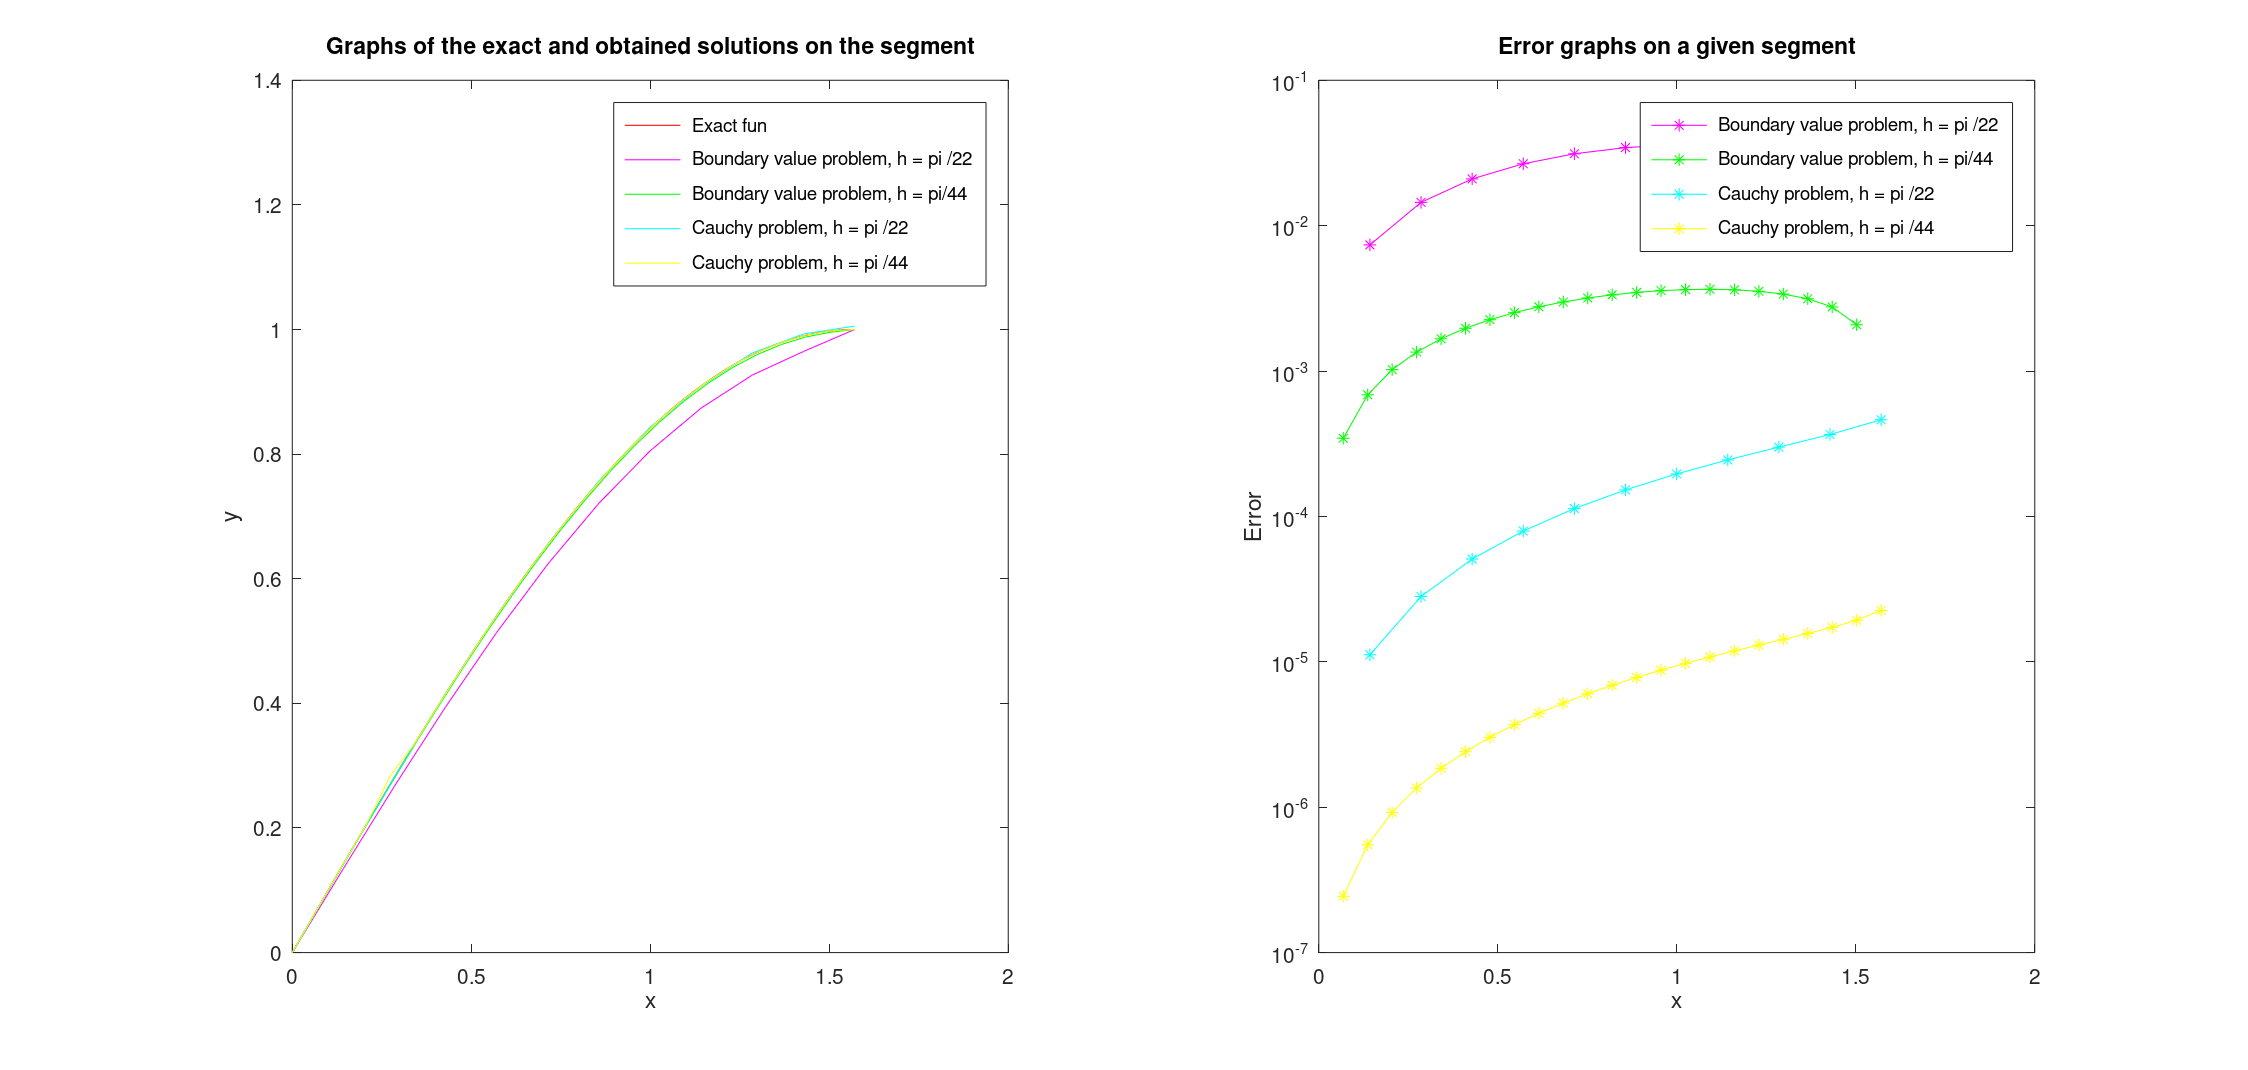
\includegraphics[width=\linewidth]{graphic1.png}
		\caption{Сравнение результатов по графикам ошибок на отрезке для двух значений
			шага}
	\end{figure}
	Заметно, что увеличение числа точек положительно сказывается на сходимости обеих
	задач. Также оба графика явно демонстрируют следующее: в задаче Коши ошибка действительно накапливается и достигает своего максимального значения на правом конце отрезка.
	В случае же краевой задачи с граничными условиями 1-ого типа ошибки на концах отрезка принимают нулевые значения, в то время как максимальная ошибка находится левее середины отрезка.

	\begin{figure}[h]
		\centering
			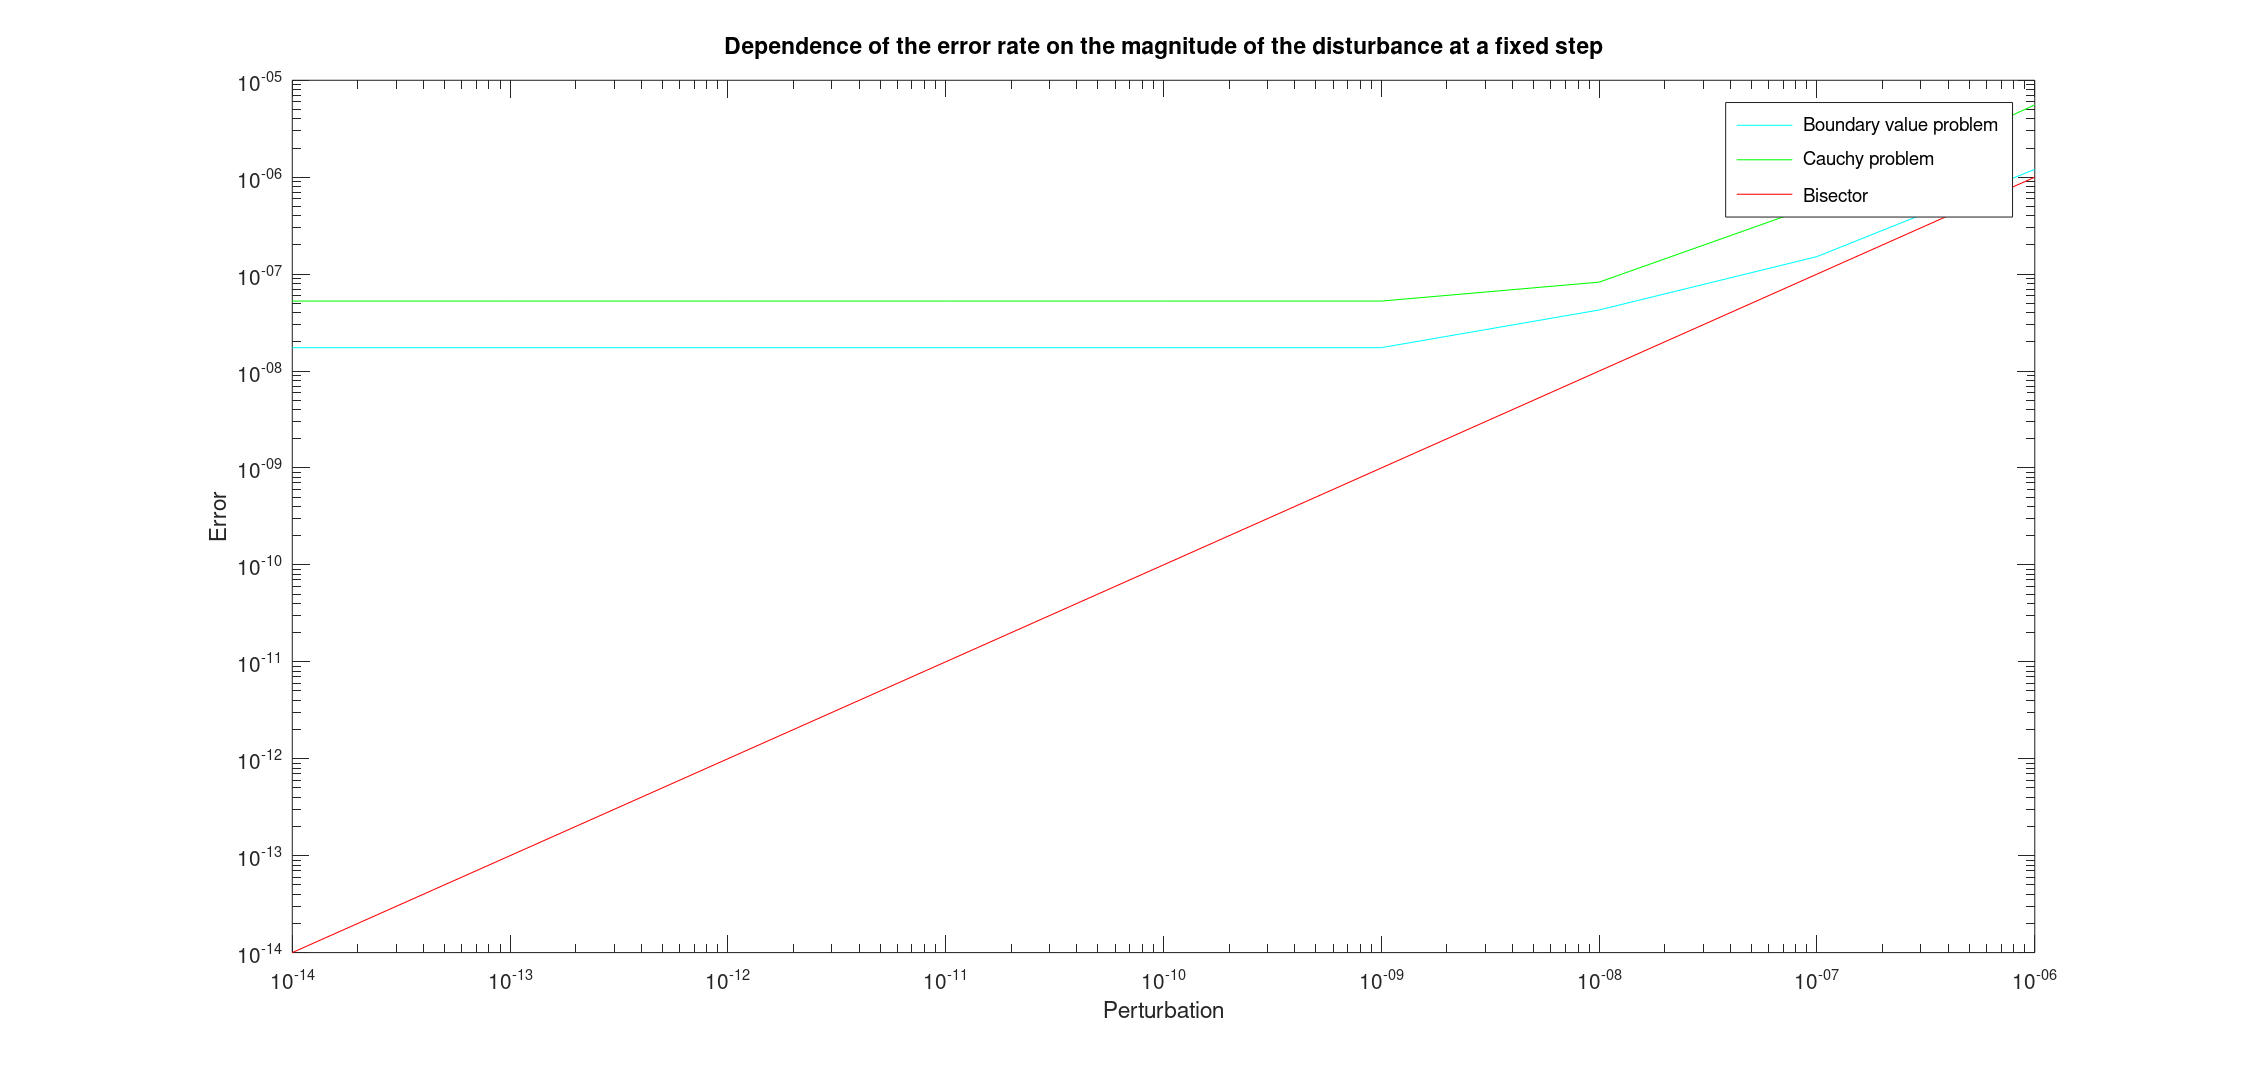
\includegraphics[width=\textwidth]{graphic2.png}
			\caption{Зависимость нормы погрешности от возмущения начальных условий при
				фиксированном шаге}
	\end{figure}
	По графику можно заметить, что при шаге $h = \frac{\pi}{2998}$ при малых возмущениях(меньше $10^{-6}$, $10^{-7}$) ошибка стабилоизировлась, и точность у краевой задачи порядка $10^{-7}$, у задачи Коши $10^{-8}$. Тем самым подтверждаются теоритические расчёты и порядки методов(точности $O(h^2), O(h^3)$ у МКР и Рунге-Кутты соответсвенно).   При больших возмущениях(больше $10^{-6}$, $10^{-7}$) как и согласно теоретиечским расчётам: ошибка при уменьшении числа возмущения в начальные условия монотонно убывает.
	\section{Выводы}
	\begin{comment}
	Задача Коши и краевая задача - два частых явления, возникаюзих как результат обработки некоторой физической или математической модели. В основе каждой из них лежит идея решения ОДУ. Погрешности же решений в случае вышеупомянутых методов различаются, что является поводом к тому, чтобы понять, к какой лучше задаче сводить модель. К примеру, если отрезок, на котором необходимо вычислить решение ОДУ, велик, и не требуется точность более чем $10^{-3}$, то ресурсов на решение краевой задачи потребуется меньше, чем на решение задачи Коши при прочих равных. Тем не менее, если же требуется более высокая точность, то в рекомендацию всупает уже метод Рунге-Кутты 4 порядка и соответствующая ему задача Коши.
	\end{comment}
	
	Проводя сравнение погрешностей для метода Рунге-Кутты и метода конечных разностей, можно говорить о следующем: как показали результаты исследований, задача Коши устойчива к возмущениям начальных данных. Получилось, что метод Рунге-Кутты более предпочтителен для обработки данных, в которых предполагается ошибка.
\end{document}